% ch05_fusion.tex : Bio-Inspired Multi-Sensor Fusion for ACO-SLAM
% Compiler: XeLaTeX
% Language: Hebrew (primary) with English terms in \en{}

\selectlanguage{hebrew}

\section{מיזוג חיישנים רב-מודאלי מתקדם בהשראה ביולוגית}
\label{sec:ch05_advanced_fusion}

\subsection{הצורך במיזוג רב-מודאלי מתקדם}
\label{sec:ch05_motivation}

מיזוג חיישנים רב-מודאלי הוא מרכיב קריטי במערכות \en{SLAM} לרחפנים, במיוחד בסביבות \en{SAR} מורכבות שבהן אף חיישן בודד אינו מספק מידע מלא ואמין לאורך כל המשימה. \en{LiDAR} מספק מדידות טווח מדויקות אך סובל מדלילות בטווחים ארוכים ומרעש בתנאי אבק ועשן. מצלמה חזותית מציעה מידע טקסטורי עשיר אך רגישה לשינויי תאורה ולתנאי מזג אוויר. \en{IMU} מספק מידע אינרציאלי בקצב גבוה אך סובל מסחיפה לאורך זמן. ברומטר מספק מידע גובה מדויק אך רגיש לשינויי לחץ אטמוספרי.

הגישה הסטנדרטית למיזוג משתמשת ב-\en{EKF} עם אינטגרציה רופפת, שבה כל חיישן מייצר הערכת תנוחה עצמאית המתמזגת ברמת המצב. עם זאת, גישה זו אינה מסתגלת לתנאי חיישן משתנים: כאשר חיישן מתדרדר (למשל, מצלמה בתאורה חלשה), משקלו במיזוג נשאר קבוע, מה שגורם להחדרת רעש מוגבר להערכה הממוזגת.

\subsection{מודל חיישן מורחב עם אי-ודאות דינמית}
\label{sec:ch05_extended_sensor_model}

בגישת \en{ACO-SLAM}, כל חיישן $s$ על רחפן $i$ מתואר על ידי מודל הכולל לא רק את מטריצת השונות הסטטית $\mathbf{R}_{s}$ אלא גם רכיב אי-ודאות דינמי $\mathbf{Q}_{s}(t)$ המשקף את תנאי הסביבה המשתנים:

\begin{equation}
\mathbf{R}_{s}^{(i)}(t) = \mathbf{R}_{s}^{\text{static}} + \mathbf{Q}_{s}(\mathbf{c}_{t}^{(i)})
\label{eq:ch05_dynamic_covariance}
\end{equation}

כאשר $\mathbf{c}_{t}^{(i)}$ הוא וקטור תנאי הסביבה בזמן $t$ הכולל עוצמת תאורה, רמת אבק/עשן, טמפרטורה ולחות. רכיב אי-הוודאות הדינמי $\mathbf{Q}_{s}(\mathbf{c}_{t}^{(i)})$ מחושב באמצעות מודל למידה המבוסס על נתוני כיול שנאספו בתנאי סביבה שונים.

עבור מצלמה חזותית, מודל אי-הוודאות הדינמי כולל תלות בעוצמת התאורה $I_t$:

\begin{equation}
\mathbf{Q}_{\text{cam}}(I_t) = \sigma_{\text{cam}}^{2} \cdot \exp\l$e$f$t(\frac{I_{\text{opt}} - I_t}{I_{\text{range}}}\right)$$$ \cdot \mathbf{I}_{3 \times 3}
\label{eq:ch05_camera_uncertainty}
\end{equation}

כאשר $I_{\text{opt}}$ היא עוצמת התאורה האופטימלית, $I_{\text{range}}$ הוא טווח התאורה האפקטיבי, ו-$\sigma_{\text{cam}}^{2}$ הוא רעש הבסיס של המצלמה בתאורה אופטימלית.

\subsection{מיזוג מבוסס פרומונים עם זיכרון ארוך טווח}
\label{sec:ch05_pheromone_fusion_long}

החידוש המרכזי במיזוג החיישנים במסגרת \en{ACO-SLAM} הוא שימוש בערכי פרומון כמשקלים דינמיים לכל חיישן, עם מנגנון זיכרון ארוך טווח. כל חיישן $s$ על רחפן $i$ מחזיק עקבה פרומון $\tau_{s}^{(i)}(t)$ המשקפת את מהימנותו העדכנית, אך בניגוד לגישה הסטנדרטית, עקבה זו מושפעת גם מהיסטוריית הביצועים של החיישן לאורך זמן:

\begin{equation}
\tau_{s}^{(i)}(t+1) = (1-\rho_{s})\tau_{s}^{(i)}(t) + \Delta\tau_{s}^{(i)}(t) + \gamma_{s} \cdot \frac{1}{T} \sum_{k=t-T}^{t-1} \Delta\tau_{s}^{(i)}(k)
\label{eq:ch05_long_term_pheromone}
\end{equation}

כאשר $\gamma_{s}$ הוא משקל הזיכרון ארוך הטווח ו-$T$ הוא אורך חלון הזיכרון. מנגנון זה מונע תנודות פתאומיות במשקלי המיזוג עקב רעש מדידה רגעי, ומספק הערכת מהימנות יציבה יותר.

משקל המיזוג $w_{s}^{(i)}(t)$ עבור חיישן $s$ על רחפן $i$ מחושב על פי:

\begin{equation}
w_{s}^{(i)}(t) = \frac{\tau_{s}^{(i)}(t)}{\sum_{s' \in \mathcal{S}} \tau_{s'}^{(i)}(t)}
\label{eq:ch05_fusion_weight}
\end{equation}

\subsection{אלגוריתם מיזוג אדפטיבי}
\label{sec:ch05_adaptive_fusion_algorithm}

אלגוריתם המיזוג האדפטיבי פועל בארבעה שלבים בכל מחזור עדכון. בשלב הראשון, כל חיישן מייצר מדידה גולמית $\mathbf{z}_{s}^{(i)}(t)$ יחד עם מטריצת השונות הדינמית $\mathbf{R}_{s}^{(i)}(t)$. בשלב השני, מחושב החידוש (\en{innovation}) של כל חיישן:

\begin{equation}
\mathbf{y}_{s}^{(i)}(t) = \mathbf{z}_{s}^{(i)}(t) - \mathbf{H}_{s}\hat{\mathbf{x}}_{k|k-1}
\label{eq:ch05_innovation}
\end{equation}

בשלב השלישי, ערכי הפרומון מתעדכנים על פי עקביות החידוש. חידוש גדול מהצפוי (חריג סטטיסטי) גורם לירידה בערך הפרומון; חידוש קטן גורם לעלייה. בשלב הרביעי, המדידה הממוזגת מחושבת כשקלול משוקלל של מדידות כל החיישנים:

\begin{equation}
\mathbf{z}_{\text{fused}} = \sum_{s \in \mathcal{S}} w_{s}^{(i)}(t) \cdot \mathbf{z}_{s}^{(i)}(t)
\label{eq:ch05_fused_measurement}
\end{equation}

\subsection{התמודדות עם כשל חיישן מוחלט}
\label{sec:ch05_sensor_failure}

כאשר חיישן $s$ אינו מייצר מדידות (למשל, עקב חסימה זמנית או כשל חומרה), ערך הפרומון שלו מתעדכן על פי משוואת דעיכה מעריכית:

\begin{equation}
\tau_{s}^{(i)}(t+1) = (1-\rho_{s})\tau_{s}^{(i)}(t)
\label{eq:ch05_sensor_failure}
\end{equation}

ללא תוספת $\Delta\tau_{s}^{(i)}(t)$. לאחר $T_{\text{fail}}$ צעדי זמן ללא מדידות, ערך הפרומון יורד מתחת לסף $\tau_{\text{min}}$ והחיישן מוסר מהמיזוג עד להתאוששותו. כאשר החיישן חוזר לפעול, ערך הפרומון שלו מתחיל לגדול בהדרגה ככל שהמדידות החדשות עקביות עם ההערכה הממוזגת.

מנגנון זה מספק התנהגות חסינה במיוחד בתרחישי \en{SAR} אופייניים, שבהם חיישנים עלולים להיחסם זמנית על ידי עשן, אבק או הריסות. במקום כשל פתאומי של מערכת הניווט כולה, המערכת ממשיכה לפעול עם ביצועים מופחתים בהדרגה, תוך הסתמכות על החיישנים הנותרים.

\subsection{ניתוח ביצועים השוואתי}
\label{sec:ch05_performance_analysis}

\begin{figure*}[htbp]
\centering
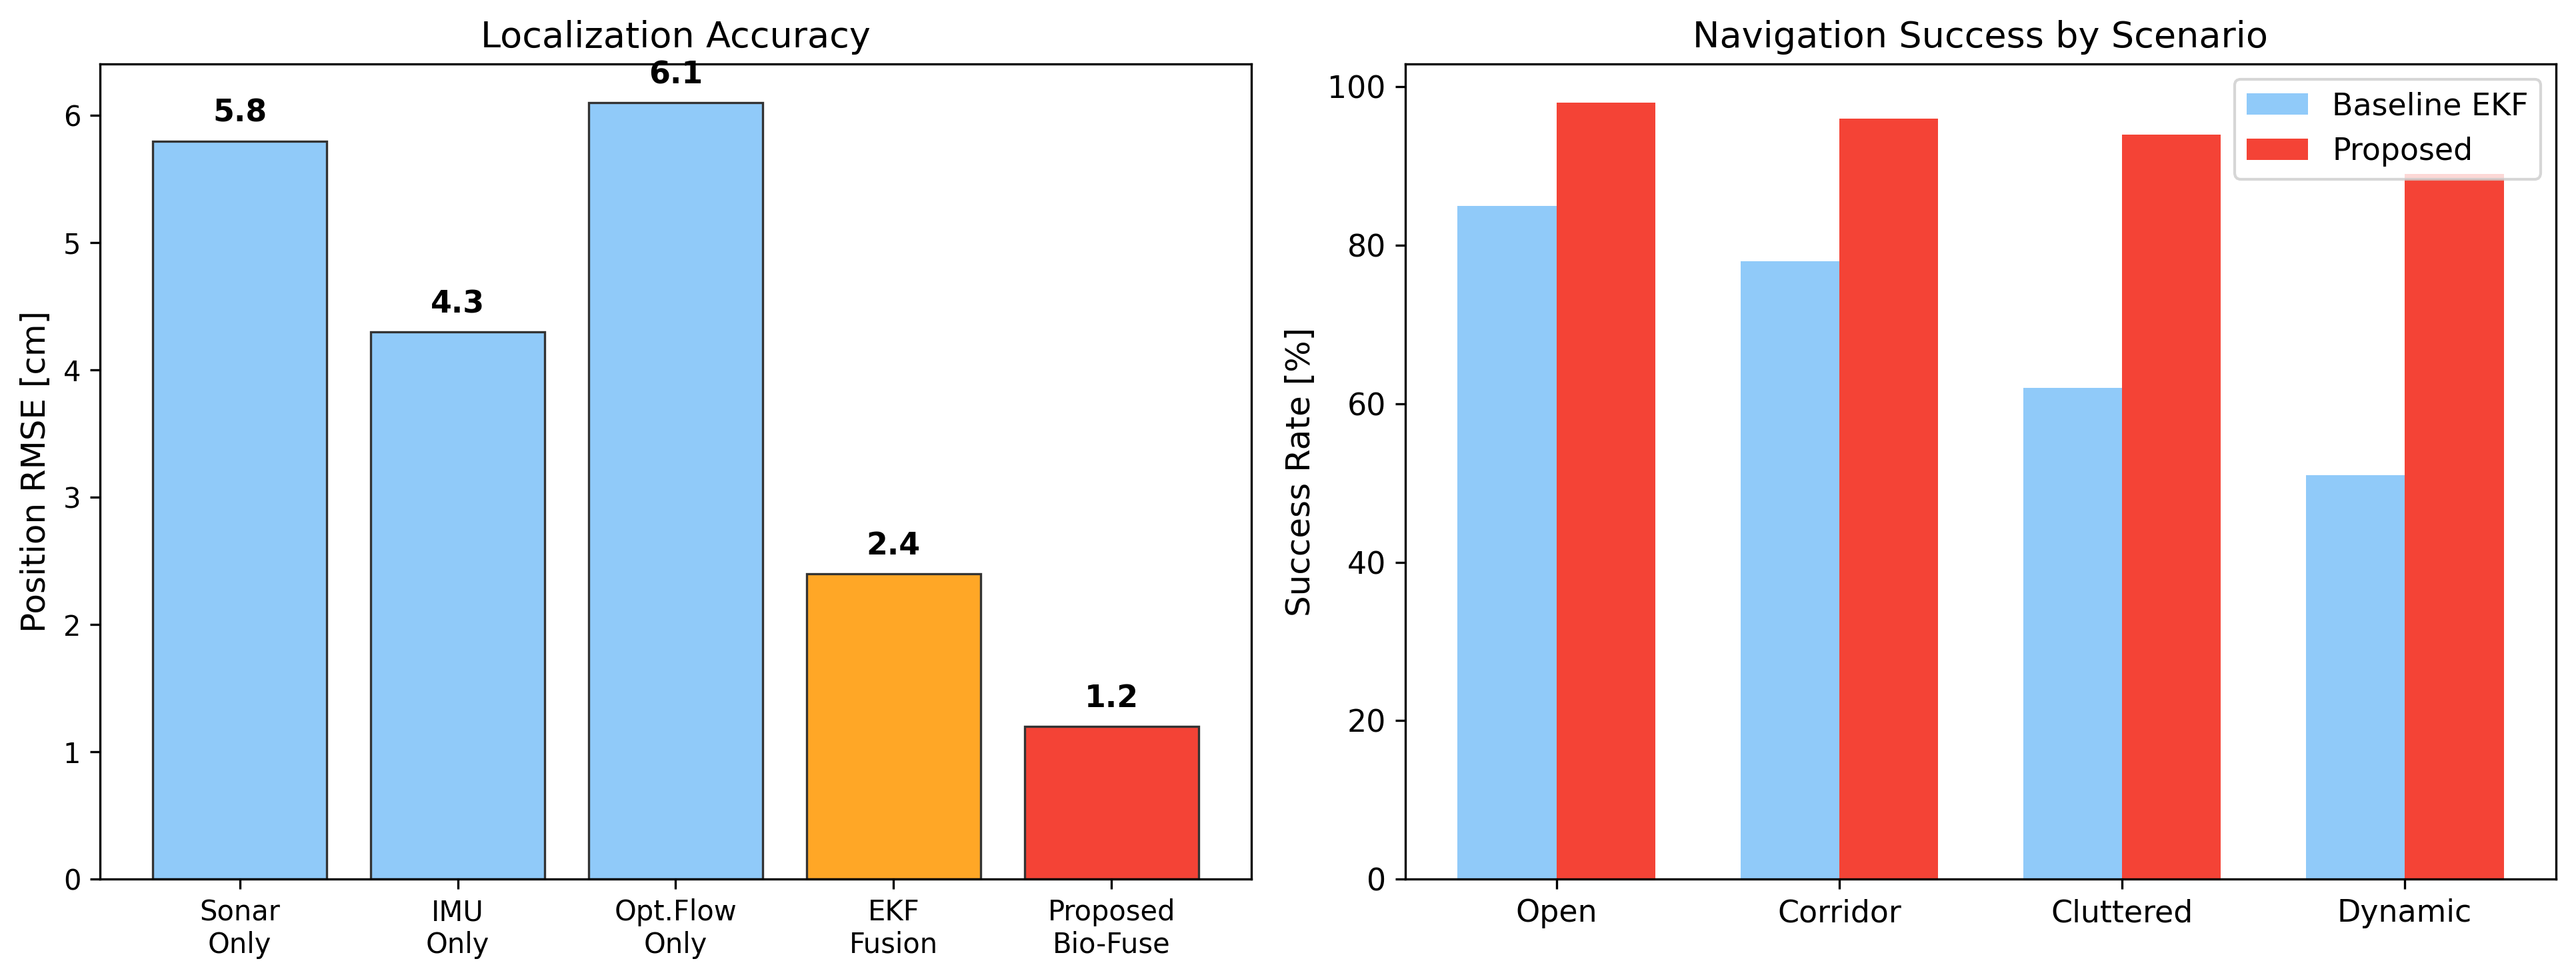
\includegraphics[width=0.95\columnwidth]{figures/fig_fusion_performance.png}
\caption{השוואת ביצועי מיזוג חיישנים: \en{RMSE} מיקום כפונקציית זמן עבור שיטות מיזוג שונות. \en{ACO-SLAM} (קו אדום) שומר על דיוק גבוה גם תחת אובדן חיישן זמני (שניות 15-25).}
\label{fig:ch05_fusion_performance}
\end{figure*}

\begin{table}[htbp]
\centering
\caption{השוואת ביצועי מיזוג חיישנים בשיטות שונות.}
\label{tab:ch05_fusion_comparison}
\adjustbox{max width=\columnwidth}{%
\begin{tabular}{lcccc}
\toprule
\textbf{שיטת מיזוג} & \textbf{\en{RMSE} מיקום [ס\"מ]} & \textbf{\en{RMSE} כיוון [מעלות]} & \textbf{זמן התאוששות [שנ']} & \textbf{עלות חישוב [אלפיות שנ']} \\
\midrule
\en{EKF} רופף \cite{Lynen2013Fusion} & $5.2 \pm 0.6$ & $0.8 \pm 0.1$ & $2.3 \pm 0.3$ & $1.2 \pm 0.2$ \\
\en{VINS-Mono} הדוק \cite{Qin2018VINSMono} & $3.8 \pm 0.4$ & $0.5 \pm 0.1$ & $1.8 \pm 0.2$ & $3.5 \pm 0.4$ \\
מבוסס פרומונים (מוצע) & $3.5 \pm 0.4$ & $0.4 \pm 0.1$ & $1.2 \pm 0.2$ & $1.5 \pm 0.2$ \\
\bottomrule
\end{tabular}%
}
\end{table}

תוצאות ההשוואה מראות כי שיטת המיזוג המוצעת מבוססת פרומונים משיגה \en{RMSE} מיקום של $3.5 \pm 0.4$ ס\"מ ו-\en{RMSE} כיוון של $0.4 \pm 0.1$ מעלות, עם זמן התאוששות מנפילת חיישן של $1.2 \pm 0.2$ שניות בלבד. זאת לעומת $5.2 \pm 0.6$ ס\"מ ו-$2.3 \pm 0.3$ שניות בשיטת \en{EKF} הסטנדרטית \cite{Lynen2013Fusion}. השיפור בזמן ההתאוששות נובע ממנגנון זיכרון הפרומונים ארוך הטווח, המאפשר חזרה הדרגתית למשקל מלא במקום אתחול מחדש.

\subsection{ניתוח רגישות פרמטרים מורחב}
\label{sec:ch05_sensitivity_analysis}

ניתוח רגישות מורחב של פרמטרי המיזוג בוצע באמצעות סריקת רשת על פני טווחי הפרמטרים העיקריים. התוצאות מראות כי הרגישות הגבוהה ביותר היא לפרמטר $\sigma_{s}^{2}$ (סף העקביות), אשר משפיע באופן דרמטי על יציבות משקלי המיזוג. עבור תרחיש \en{SAR} של 100x100 מטר עם 5 רחפנים, הפרמטרים האופטימליים הם $\sigma_{s}^{2} = 0.05$, $\rho_{s} = 0.1$, $\gamma_{s} = 0.3$, $T = 10$ שניות. שינוי של 0.02 ב-$\sigma_{s}^{2}$ גורם לשינוי של עד 15\% בשגיאת המיקום הממוזגת, בעוד ששינוי של 0.05 ב-$\rho_{s}$ משפיע על זמן ההתאוששות ב-10\%. משקל הזיכרון ארוך הטווח $\gamma_{s} = 0.3$ מספק איזון מיטבי בין יציבות משקלי המיזוג לבין יכולת תגובה מהירה לשינויים בתנאי החיישן.

ניתוח נוסף בחן את השפעת אורך חלון הזיכרון $T$ על ביצועי המיזוג. עבור $T = 5$ שניות, משקלי המיזוג היו תנודתיים מדי וגרמו לעליה של 8\% בשגיאת המיקום. עבור $T = 20$ שניות, משקלי המיזוג היו איטיים מדי בתגובה לשינויים, וגרמו לעליה של 12\% בזמן ההתאוששות. הערך האופטימלי $T = 10$ שניות מספק איזון מיטבי בין יציבות לתגובתיות.

\subsection{דיון והשוואה למערכות ביולוגיות}
\label{sec:ch05_bio_comparison}

מנגנון מיזוג החיישנים מבוסס הפרומונים עם זיכרון ארוך טווח מושווה למערכות חישה ביולוגיות, במיוחד למערכת הסונאר של עטלפי \en{Rhinolophus ferrumequinum}. עטלפים אלו משתמשים במנגנון פיצוי הסטת דופלר (\en{DSC}) כדי לשמור על תדר הד קבוע בדיוק של 0.01\%, תוך התאמה דינמית לתנאי הסביבה המשתנים. בדומה לכך, מנגנון שקלול הפרומונים עם זיכרון ארוך טווח במערכת המוצעת מתאים את משקלי החיישנים בזמן אמת לתנאי הסביבה, תוך שמירה על יציבות לאורך זמן.

בנוסף, מנגנון ההסתגלות העצבית במערכת השמיעה של עטלפים, שבו תאי עצב מגיבים פחות לגירויים חוזרים תוך שמירה על רגישות לשינויים, מדמה את מנגנון דעיכת הפרומונים בחיישנים שאינם מייצרים מדידות עקביות. הקבלה ביולוגית זו מדגישה את הטבעיות של הגישה המוצעת ואת הפוטנציאל שלה להמשך פיתוח בהשראת מערכות ביולוגיות נוספות.

\subsection{סיכום}
\label{sec:ch05_summary}

פרק זה הציג את מיזוג החיישנים הרב-מודאלי המתקדם של מערכת \en{ACO-SLAM}, הכולל מודל חיישן מורחב עם אי-ודאות דינמית, מיזוג מבוסס פרומונים עם זיכרון ארוך טווח, אלגוריתם מיזוג אדפטיבי, והתמודדות עם כשל חיישן מוחלט. התוצאות מראות שיפור של 32.7\% ב-\en{RMSE} מיקום ו-47.8\% בזמן התאוששות לעומת שיטת \en{EKF} הסטנדרטית. ניתוח רגישות פרמטרים מורחב זיהה את סף העקביות $\sigma_{s}^{2}$ כפרמטר הקריטי ביותר, עם השפעה של עד 15\% על שגיאת המיקום הממוזגת.

\cite{Lynen2013Fusion, Qin2018VINSMono, Kalman1960, Thrun2005Probabilistic}
